% 自分用LaTeXテンプレート
% タイプセットはupLaTeX, dvipdfmxを使用,スタイルはjsarticle

\documentclass[uplatex, a4paper]{jsarticle}
\usepackage[dvipdfmx]{graphicx}

\usepackage{tabularx}   % 表
\usepackage{layout}     % レイアウト

% ---数式関係---
\usepackage{amsmath}    % ams math
\usepackage{bm}         % ボールド

\usepackage{url}    % URLを書くため
\usepackage{siunitx}    % SI単位を書くため

\usepackage[dvipdfmx]{xcolor}   % 色指定
\usepackage{listings} % コードブロック
\lstset{
  basicstyle = \small\ttfamily,
  keywordstyle = \color[RGB]{33, 150, 243},
  commentstyle = \color[RGB]{76,175,80},
  backgroundcolor = \color[gray]{.95},
  breaklines = true,
  breakautoindent = true,
  captionpos = t,
  keepspaces = true,
  columns = flexible,
  showspaces = false,
  showstringspaces = false,
  showtabs = false,
  aboveskip = 6pt,
  belowskip = 6pt,
  xleftmargin = 10pt,
  xrightmargin = 10pt,
  frame = tb,
  framesep = 8pt,
  framerule = 0.1pt,
  frameround = tttt,
  framexleftmargin = 10pt,
  framexrightmargin = 10pt,
  rulecolor = \color[gray]{.95},
  tabsize = 2
}

%\pagestyle{empty}  % ページ番号消去
\pagestyle{plain}   % ページ番号表示

% ---レイアウトパラメータ---
\usepackage[left=25mm,right=25mm,top=20mm,bottom=20mm, includefoot]{geometry}

\def\Vec#1{\mbox{\boldmath $#1$}}   % ベクトル(ボールド)の定義

\renewcommand{\tablename}{Table}    % 表番号フォーマットをTableへ
\renewcommand{\figurename}{Fig.}    % 図番号フォーマットをFig.へ

\renewcommand{\lstlistingname}{Code}  % コードブロックのキャプションを"Code"に変更

\renewcommand{\baselinestretch}{0.8}    % 行間の調整
\renewcommand{\arraystretch}{1.2}       % 表の行高さの調整

\title{\Huge タイトル} 
\author{\huge 書いた人の名前}
\date{\today}

% ---ドキュメント開始---
\begin{document}

\maketitle  % タイトル生成

\section{テンプレート}
ここに本文を書く.これは自分用のテンプレートです.

\section{なんでupLaTeXなの?}
研究室での \LaTeX の形式がこれだったから

%input{Folder/documentname.tex} % ファイルをインポート

\subsection{使い方}
  \begin{itemize}
      \item このテンプレートには各種設定や基本的なコマンドの使い方などが含まれます
      \item 不要な部分は削除してお使いください
      \item やる気がある限り順次更新されていくと思います
  \end{itemize}

図はPDF形式で貼りましょう.図\ref{fig:sample}はサンプル画像です.

  % 図を貼る
  \begin{figure}[h]   % h: この場所に t: ページのトップに b: ページのボトムに p: 新しいページを作って画像を貼る
      \centering              % 中央揃え
      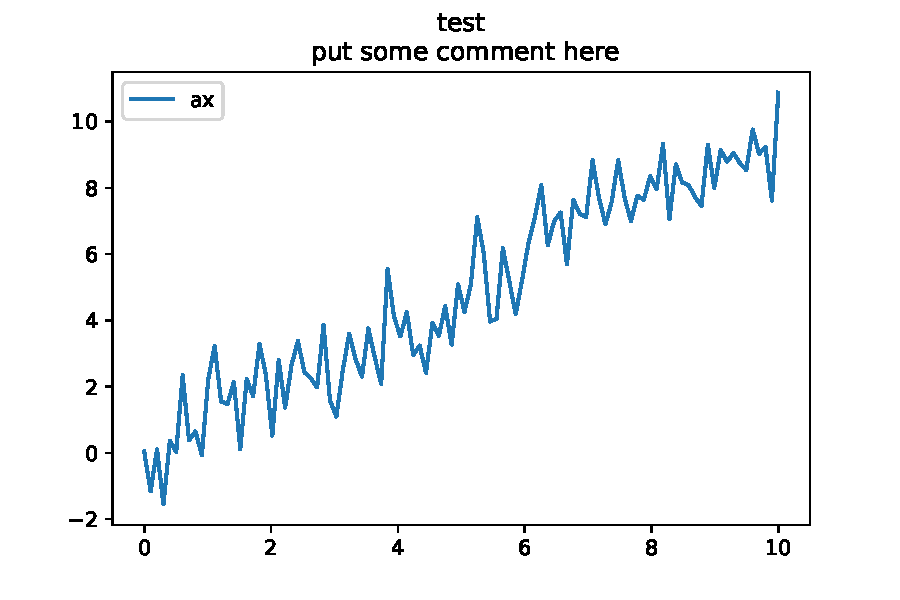
\includegraphics[width=60truemm,clip]{images/graph_sample.pdf}
      \caption{Sample Picture}% 図のタイトル(英語)
      \label{fig:sample}      % 参照用ラベル
  \end{figure}

  図を横に並べて貼ることもできます.自動改行を防ぐために\textsf{tabular}環境を使います.

  % 横に並べて図を貼る(自動改行を防ぐためにtabularを使う)
  \begin{figure}[h]
    \begin{center}    % 中央揃え
      \begin{tabular}{c}
        \begin{minipage}{.45\linewidth}   % 左側の図
        \centering
        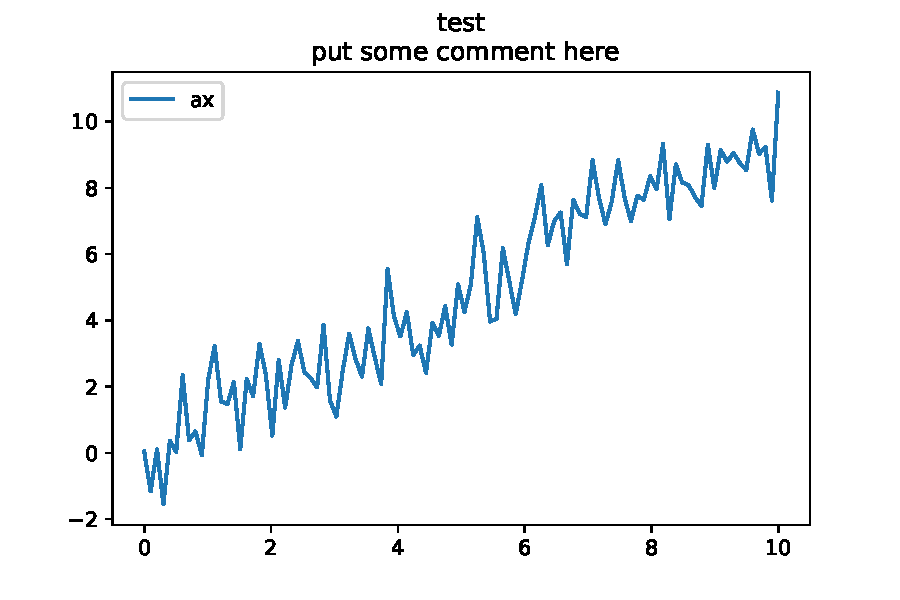
\includegraphics[width=60truemm,clip]{images/graph_sample.pdf}
        \caption{Sample Picture(Left side)} % 図のタイトル(英語)
        \label{fig:sample_l}                % 参照用ラベル
        \end{minipage}
        
        \begin{minipage}{.45\linewidth}   % 右側の図
        \centering
        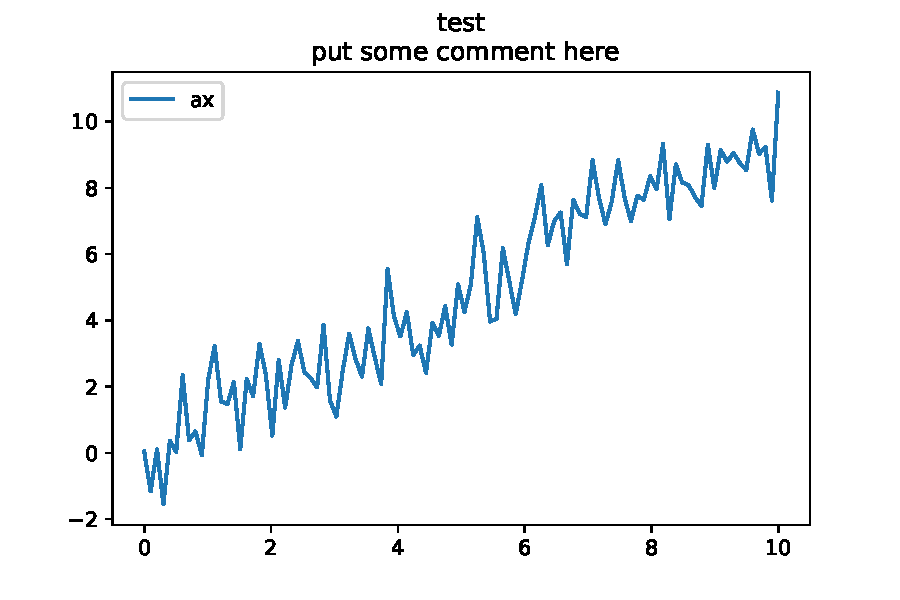
\includegraphics[width=60truemm,clip]{images/graph_sample.pdf}
        \caption{Sample Picture(Right side)}% 図のタイトル(英語)
        \label{fig:sample_r}                % 参照用ラベル
        \end{minipage}
      \end{tabular}
    \end{center}
  \end{figure}

  \LaTeX で表を書くには\textsf{table}環境と\textsf{tabular}環境を使用します.

  % 表を書く
  \begin{table}[h]
    \begin{center}
      \caption{表のサンプル}
      \begin{tabular}{|c||c|c|c|c|} \hline
        $i$ & $a_{i}$ & $\alpha_{i}$  & $d_{i}$  & $\theta_{i}$             \\ \hline \hline
         1  &    0    &       0       &    0     & $\theta_{1}$             \\ \hline
         2  &    0    & $-90^{\circ}$ &    0     & $\theta_{2}$             \\ \hline
         3  & $l_{3}$ &       0       &    0     & $\theta_{3}$             \\ \hline
         4  & $l_{4}$ &       0       &    0     & $\theta_{4}+90^{\circ}$  \\ \hline
         5  &    0    & $-90^{\circ}$ &    0     & $\theta_{5}$             \\ \hline
         6  &    0    &       0       & $-l_{5}$ &    0                     \\ \hline
      \end{tabular}
      \label{tab:dhparameter}
    \end{center}
  \end{table}

  数式は\textsf{amsmath}パッケージによって提供されています.
  オーソドックスな数式は\textsf{equation}環境を使って書くことができます.

  % 数式を書く
  \begin{equation}
  {}^0\!T_{1}=\begin{pmatrix} C_{1} & -S_{1} & 0 & 0 \\ S_{1} & C_1 & 0 & 0 \\ 0 & 0 & 1 & 0 \\ 0 & 0 & 0 & 1 \end{pmatrix}
  \end{equation}

  数式にラベルを付けて,参照することもできます.
  式\ref{eq:gaussian}は標準正規分布の公式です.

  \begin{equation}
    f(x)=\dfrac {1}{\sqrt{2\pi}\sigma}\exp\biggl\{ -\dfrac {(x-\mu)^2}{2\sigma^2}\biggr\}, \quad -\infty<x<\infty
    \label{eq:gaussian}
  \end{equation}

  コードブロックを記述することもできます.
  ただしPDFの仕様上,コピペには向きません.ご注意ください.
  また,\textsf{lstlisting}環境のインデントも反映されてしまうので,\LaTeX ソースコードのインデントが少し乱れます.
  それは仕様と割り切って我慢しましょう.

\begin{lstlisting}[language=sh]
# hogehoge
sudo apt update
sudo apt upgrade \
  curl \
  && hoge
cd ~/Documents
\end{lstlisting}

  コードブロックにはキャプションやラベルを付けることができます.

\begin{lstlisting}[caption=Generic Language Code Block, label=code:hoge]
hogehoge
hoge: moge
\end{lstlisting}

  コードブロック\ref{code:hoge}は言語オプションを指定していません.
  シンタックスハイライトは全て無効化されます.

\end{document}
% --- ドキュメント終了 ---
